\documentclass[a4paper, 12pt]{scrartcl}
\usepackage[utf8]{inputenc}
\usepackage[ngermanb]{babel}
\usepackage{setspace}
\usepackage{geometry}
\usepackage{graphicx}
\usepackage{cite}
\usepackage{amsmath}
\geometry{a4paper, top=25mm, left=25mm, right=25mm, bottom=25mm}

\title{Seminar IT-Sicherheit}
\author{Kevin Seidel \\ Studiengang Informatik \\ Matrikelnummer: 943147}

\begin{document}
\begin{titlepage}
\begin{center}
\vspace*{1.5cm}
\begin{Large}
\textbf{Universität Osnabrück}
\end{Large}

\noindent\hrulefill
\\[3.5cm]
PRAKTIKUMSBERICHT \\[1cm]
zum Programmierpraktikum \\[1cm]
\textbf{Paralelle Algorithmen mit OpenCL} \\[1.5cm]
im Sommersemester 2013 \\[1.5cm]
Thema: \\[0.5cm]
\textbf{Voxelization} \\[2cm]
Erstellt am 25.10.2013
\end{center}
\vfill
\begin{flushleft}
Vorgelegt von: 
\hfill \parbox{46mm}{Kevin Seidel} \\
\hfill \parbox{46mm}{943147} \\
\hfill \parbox{46mm}{Falkenstra"se 43} \\
\hfill \parbox{46mm}{49124 Georgsmarienh"utte}
\end{flushleft}
\end{titlepage}

\newpage

\pagenumbering{Roman}
\setcounter{page}{2}
\tableofcontents

\newpage
\pagenumbering{arabic}
\setcounter{page}{1}

\section{Einleitung}
W"ahrend des Praktikums habe ich mich mit der Voxelization von Szenen auf der GPU besch"aftigt. Dabei geht es darum, eine aus Polygonen bestehende Szene in ein Voxelgatter zu "uberf"uhren. Um diese Aufgabe in Echtzeit auszuf"uhren, wird daf"ur die Grafikkarte genutzt, da diese, auf Grund ihrer hohen Paralellit"at, sehr gut daf"ur geeignet ist.
Die gewonnenen Voxeldaten k"onnen danach f"ur die Beleuchtung der Szene verwendet werden. Dadurch ist es beispielsweise m"oglich die indirekte Beleuchtung, Spiegelungen oder die Ambient Occlusion einer Szene in Echtzeit zu berechnen und das zu einem sehr guten Ergebnis.
Im weiteren Verlauf dieses Berichts wird auf zwei verschiedene M"oglichkeiten der Voxelizierung eingegangen. Zum einen die Durchf"uhrung der Voxelization mittels OpenGL und zum anderen mittels OpenCL.
Ausserdem wird noch ein effizentes Speichermodell der Voxeldaten, der sogenannt Sparse Voxel Octree vorgestellt, welcher sowohl eine kompakte Speicherung der Daten als auch einen schnellen Zugriff auf die gespeicherten Voxeldaten erlaubt. 
Abschlie"send wird noch auf die weitere Nutzung der erzeugten Voxeldaten eingegangen, speziell auf die indirekte Beleuchtung einer Szene.

\section{Voxel und Voxelization}
\subsection{Voxel}
Das Wort Voxel setzt sich aus den englischen Begriffen ''volumetric'' und ''pixel'' zusammen. Frei "ubersetzt kann man es als einen dreidimensionalen Pixel bezeichnen.
Das Voxel hat im Allgemeinen nur zwei Eigenschaften, welche dem eines Pixels gleichkommen. Es besitzt eine Position in einem vorher festgelegtem, dreidimensionalen Raum und einen Farbwert.
Dieser 3D-Raum ist dabei, in jede Richtung, in gleichm"a"sige Koordinaten aufgeteilt.
F"ur meinen Verwendungszweck wird das Voxel als W"urfel dargestellt, wobei alle Seiten die Farbe des Voxels tragen.
\subsection{Voxelization}
Die Voxelization ist die "Uberf"uhrung einer Szene aus Polygonen in ein Voxelgitter, wobei f"ur jedes Voxel bestimmt wird, ob es von einem Polygon "uberschnitten wird oder nicht.

Bei der Voxelization gibt es verschiedene Verfahren. Zum einen die Oberfl"achen-Voxelization,  welche nur direkte "Uberschneidung der Polygone mit Voxeln im Gitter erfasst. Es wird also nur die Oberfl"ache der Modelle, welche aus den Polygonen zusammengestzt sind,  ber"ucksichtigt.

Eine andere Methode ist die solide Voxelization, welche testet, ob ein Voxel innerhalb eines Objekts liegt. Dadurch werden Modelle innerhalb der Szene komplett ausgef"ullt, was man ich Abbildung 1 sehr gut erkennen kann.

\begin{figure}[h]
	\centering
		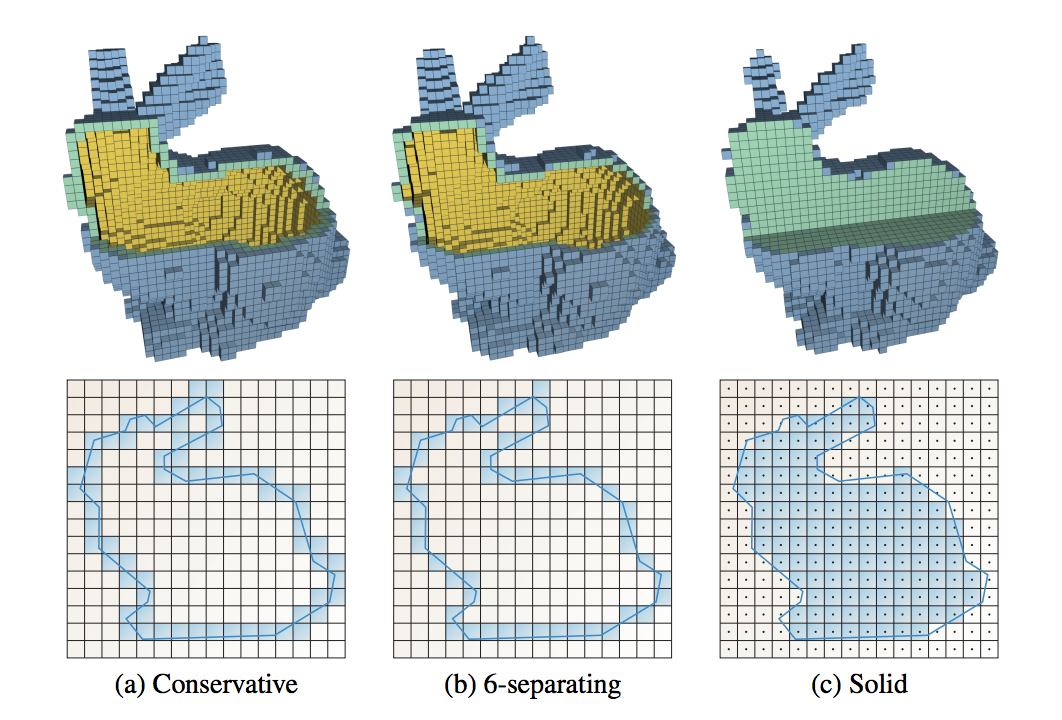
\includegraphics[width=14cm]{Kinds-of-Voxelization}
	\caption{Verschiedene Arten der Voxelization}
\end{figure}

F"ur die Nutzung der Voxel zur Beleuchtung reicht jedoch eine Oberfl"achen-Voxelization aus, so dass im weiteren Verlauf nur darauf eingegangen wird.

Die Aufgabe der Voxelization kann hochgradig paralell ausgef"uhrt werden, wodurch sich die Nutzung der GPU f"ur dieses Verfahren anbietet. In der Literatur zu diesem Problem gibt es mehrere L"osungsans"atze. 
In sehr fr"uhen Arbeiten, wo die Nutzung der ''compute mode'' der Grafikkarte noch nicht m"oglich war, wurde die Szene in mehrere Ebenen, entsprecht der Gr"o"se des Voxelgitters, zerlegt, sodass jede Voxelebene seperat gerendert wurde. Danach wurde in jeder einzelnen Ebene auf "Uberschneidungen getestet. Dies f"uhrte dazu, dass diese Verfahren sehr langsam war, da f"ur h"ohere Dimensionen sehr viele Renderaufrufe durchgef"uhrt werden mussten.

Eine etwa neuere Taktik nutzt die Paralellisierbarkeit dieser Aufgabe aus und "uberpr"uft Kollisionen zwischen den Polygonen und den Voxeln mittels GPU-Computing. Dieser Ansatz kann sowohl mittels Cuda als auch mittels OpenCL realisiert werden.
Bei dieser neueren Methode wird f"ur jedes Polygon in der Szene ein eigener Thread gestartet.
Innerhalb dieses Threads wird "uberpr"uft, ob das Polygon ein Voxel "uberschneidet. Das Ergebnis wird anschlie"send in einen Buffer geschrieben, wobei dieser f"ur jede Stelle des Voxelgrids einen Wert enth"alt, welcher angibt, ob das Voxel gef"ullt ist oder nicht. 
Zus"atzlich k"onnen auch noch andere Werte, wie Farbe oder Materialbeschaffenheit gespeichert werden.

Ein weiterer, neuerer Ansatz nutzt f"ur die Bestimmung der Voxel die feste OpenGL-Pipeline, im genaueren den Hardware-Rasterizer. Dies erm"oglicht eine noch k"urzere Laufzeit, bringt jedoch auch einige Probleme mit sich, welche bei dem OpenCL-Ansatz nicht auftreten.

Die beiden Ans"atze mittels OpenGL und OpenCL werden in weiteren Verlauf genauer erl"autert.

\newpage

\section{Voxelization mit Hilfe von OpenGL}
Zuerst habe ich mich mit der Voxelization mittels OpenGL besch"aftigt. Dieser Ansatz ist eine neuere Methode, da hierbei Funktionen aus OpenGL 4.2 genutzt werden, welches im August 2012 ver"offentlicht wurde.
Der OpenGL-Ansatz nutzt hierbei die feste Hardware-Pipleline der Grafikkarte aus, um den Prozess der Voxelization zu beschleunigen. 
Der Vorteil dieser Methode ist, dass hier nur einen einzigen Render-Durchlauf ben"otigt wird, um die komplette Szene in Voxel zu "uberf"uhren.
In diesem Ansatz wird im spezifischen der Hardware-Rasterizer genutzt, um die "Uberschneidung der Polygone und der Voxel zu bestimmen. 

Ein Problem, welches hierbei auftaucht, ist, dass der Rasterizer eigentlich dar"ur gedacht ist, eine zwei-dimensionale Szene zu rastern. F"ur das hier vorliegende Problem muss jedoch eine dreidimensionale Szene gerastert beziehungsweise voxelisiert werden.

Um dieses Problem zu l"osen, wird das Polygon, mittels Paralellprojektion, auf eine zweidimensionale Ebene projeziert.
Die Zielebene wird so gew"ahlt, dass das Polygon die gr"o"st m"ogliche Fl"ache auf dieser Ebene einnimmt.
Im dreidimensionalen Raum kommen daf"ur drei Ebenen in Frage. 
Um die geeignete Ebene zu finden, bestimmt man die dominante Achse der Normalen. 
Die dominanten Achse ist die, in welche der Normalenvektor die h"ochste Ausdehnung aufwei"st.
Ist beispielsweise die dominanten Achse die x-Achse, w"are die zu w"ahlende Ebene, die yz-Ebene.

Diese Projektion auf eine 2D-Ebene geschieht, individuell f"ur jedes Polygon, im Geometry-Shader des jeweiligen Renderaufrufs.
Hierdurch wird die gr"o"st m"ogliche Fl"ache des Dreiecks rasterisiert, wodurch m"ogliche L"ucken in der Voxelization reduziert werden. Durch die Rasterisierung erh"alt man die Pixel, welche vom Polygon "uberlappt werden. 

Um diese zweidimensionalen Positionsinformationen nun in Voxel zu "uberf"uhren, werden die Pixel nun, entgegen der zuvor bestimmten dominanten Achse, zur"uck projeziert, sodass sich die Positionsinformation nun im dreidimensionalen Raum befinden. Dadurch erh"alt man die resultierende Position der einzelnen Voxel.

\begin{figure}[h]
	\centering
		\includegraphics[width=16cm]{Voxelization-Pipeline}
	\caption{Schritte der Voxelization mittels OpenGL}
\end{figure}

Die entstehenden Voxel werden dann, mittels der in OpenGL 4.2 eingef"uhrten Methode, ''image store'', welche es erlaubt an eine beliebige Stelle in einer Textur zu schreiben, in eine 3D-Textur geschrieben. Dieser Vorgang geschieht dabei im Fragment Shader. Hierbei wird die Position des Voxels und dessen Farbwert, in die vorher erstellte 3D-Textur, geschrieben.


Mittels dieser Textur l"asst sich nun auf die Voxelinformationen zugreifen. Die Voxel lassen sich zum Beispiel direkt zeichnen. Es ist jedoch auch m"oglich zu "uberpr"ufen, ob ein Voxel vorhanden ist und welche Farbe er besitzt.

Eine Schw"ache dieser Methode ist, dass es vorkommen kann, dass auf Grund der n"otigen Projektion einige Voxel nicht registriert werden, das hei"st eine "Uberschneidung wird nicht erkannt. Dies ist darauf zur"uckzuf"uhren, dass bei der Rasterisierung mittels des Hardware-Rasterizers, nur die "Uberschneidungen am Mittelpunkt des Pixel getestet werden. 
Eine L"osung f"ur dieses Problem ist die ''konservative Rasterisierung''.
Dabei erfolgt eine Vergr"o"serung des Polygons, sodass es an jeder Ecke um $1/2$ Pixelgr"o"se beziehungsweise Voxelgr"o"se erweitert wird. Dadurch wird nun der Mittelpunkt des Pixel "uberdeckt, wo ansonsten nur die Ecken des Pixels tangiert worden w"are.

\begin{figure}[h]
	\centering
		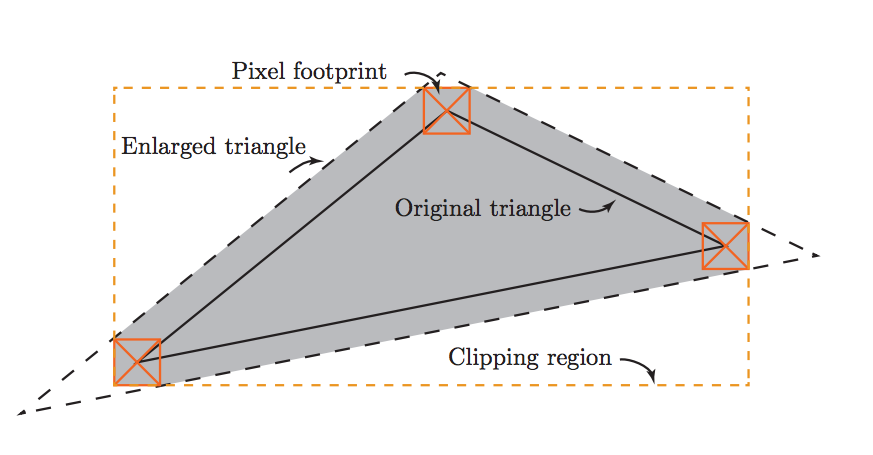
\includegraphics[width=16cm]{conservative-rasterisation}
	\caption{Beispiel f"ur konservative Rasterisierung}
\end{figure}


\newpage

\section{Voxelization mit Hilfe von OpenCL}
Bei der Voxelization mittels OpenCL muss die Erkennung von "Uberschneidungen individuell programmiert werden, da hier nicht auf einen feste Pipeline zur"uckgegriffen werden kann. Dies erlaubt jedoch auch mehr Freiheiten bei der Erkennung, Verarbeitung und Speicherung der Voxeldaten. 

Bei der "Uberf"uhrung von Polygonen in Voxel mittels eines OpenCL-Kernels wird f"ur jedes Polygon der zu voxelisierenden Szene ein eigener Thread gestartet, sodass alles Polygone paralell bearbeitet werden. 
In jedem Kernelaufruf wird daf"ur auf die "Uberschneidung zwischen dem jeweiligen Polygon und den Voxeln getestet. 
Das hei"st in jedem Kernel muss theoretisch f"ur jedes Voxel der Szene auf eine "Uberschneidung getestet werden.
Um diesen Vorgang zu beschleunigen, wird nur in der in Frage kommenden Bounding-Box des aktuellen Dreiecks auf "Uberdeckung getestet.

Das hei"st, es werden zuerst die Eckpunkte einer Box berechnet, welche das Dreieck genau umschlie"sen w"urde. Dadurch muss nicht die komplette Szene auf "Uberschneidungen getestet werden, 
F"ur jedes Voxel ,innerhalb dieser Box, wird nun getestet, ob sich ein oder mehrere Eckpunkte des Voxels auf verschiedenen Seiten eines Polygons befinden. Dadurch werden die Voxel bestimmt, welche sich auf den Seiten oder Ecken des Polygons befinden.

Des Weiteren wird f"ur jede 2D-Projektion eine Polygon und eines Voxels auf eine "Uberschneidung dieser beiden getestet.

Erst wenn beide Test erfolgreich waren, ist eine "Uberschneidung best"atigt und diese Voxel k"onnen gespeichert werden.

Dabei ist die Speicherung der Voxel bei diesem OpenCL-Ansatz frei w"ahlbar. 
In meinem Ansatz wurden alle Voxel in einen eindimensionalen Buffer geschrieben. 

\begin{figure}[h]
	\centering
		$Buffer: \begin{pmatrix}x0 \\ y0 \\ z0 \end{pmatrix}, \begin{pmatrix}x0 \\ y0 \\ z1 \end{pmatrix}, ..., \begin{pmatrix}x0 \\ y0 \\ z511 \end{pmatrix}, \begin{pmatrix}x0 \\ y1 \\ z0 	\end{pmatrix}, ..., \begin{pmatrix}x511 \\ y511 \\ z511 \end{pmatrix}$
	\caption{Aufbau des Buffers f"ur ein Voxelgrid der Dimension $512^3$}
\end{figure}

Es w"are, auf Grund der Freiheit welche die Verwendung eines eigenen OpenCL-Kernels zur Verf"ugung stellt, jedoch auch m"oglich die Voxeldaten direkt in einen Sparse Voxel Octree zu schreiben, wodurch keine weitere Umwandlung der Datenstruktur mehr n"otig ist, da der Sparse Voxel Octree schon die gewollte Speicherstruktur ist. Auch andere Speicherarten w"aren problemlos m"oglich.

Dies wurde hier jedoch, auf Grund der zus"atzlichen Komplexit"at, nicht durchgef"uhrt.

Auf den resultierenden Buffer lassen sich nun weitere Test und Methoden anwenden, welche f"ur die passive Beleuchtung n"otig sind. Es w"are jedoch auch denkbar, die Voxel direkt auszugeben.

\newpage

\section{Vergleich zwischen OpenGL und OpenCL Ansatz}
Wie bereits erw"ahnt, liegt der Hauptunterschied beider Varianten an der Nutzung der festen Hardware der Grafikkarte. 
Der Ansatz mittels OpenGL erlaubt, auf Grund der Nutzung dieser festen Hardware eine schnellere Ausf"uhrung der Voxelization.
Dies ist besonders im Bezug auf die Nutzung von schw"acherer Hardware, zum Beispiel auf mobilen Ger"aten, zu bevorzugen, jedoch auch auf performanter Hardware ein guter Ansatz.

Der Vorteil der OpenCL-Variante ist die gr"o"sere Freiheit und Anpassbarkeit bei der Voxelization, da man seinen OpenCL-Kernel nach eigenen Vorstellungen erstellen und modifizieren kann.
So l"asst sich eineigener Kernel mit individueller Voxelerkennung, Datenverarbeitung und Datenspeicherung erstellen. 
Somit ist es m"oglich die Voxelization komplett nach den eigenen Bed"urfnissen anzupassen, wobei man jedoch immer die Performanz ber"ucksichtigen sollte, welche bei sehr komplexen Kerneln leiden k"onnte und somit den Echtzeitanspruch zunichte macht.

Im direkten Vergleich l"asst sich somit keine "uberlegende Variante bestimmen, da beide sowohl Vorteile als auch Nachteile haben. 
Im Hinblick auf die Umsetzung und Programmierung dieser Methoden l"asst sich sagen, dass der OpenGL-Ansatz, im Gegensatz zur OpenCL-Variante, deutlich komplexer und schwieriger zu implementieren ist.



\section{Speicherung der Voxeldaten}
Bei der Speicherung der Voxeldaten kommt es vorallem auf zwei wichtige Faktoren an.
Zum einen soll die Nutzungsgeschwindigkeit beschleunigt werden und zum anderen soll der Speicherbedarf m"oglichst gering gehalten werden.
Dazu werden die Voxel in sogenannten Sparse Voxel Octrees gespeichert. 
Ein Octree ist eine Baumstruktur, wobei jeder Knoten jeweils acht Kindknoten hat. Diese Struktur ist hier bestens geeignet, da bei der Aufteilung eines W"urfels in gleichm"a"sige St"ucke, acht neue W"urfel entstehen, als f"ur jeden neuen W"urfel ein neuer Kindknoten erzeugt wird.

Ein weiterer Vorteil der Sparse Voxel Octrees ist, dass der entstehende Baum nicht gleichm"a"sig aufgebaut sein muss. 
Das hei"st, dass jeder Teilbaum eine beliebige Tiefe aufweisen kann.
So lassen sich zusammenh"angende Voxel des gleichen Typ (z.B. Farbe) zusammenfassen und der Baum muss nicht weiter in die Tiefe wachsen.
Diese Methode spart zum einen Speicherplatz, da nicht zwingend f"ur jedes Voxel ein Wert vorgehalten werden muss, sondern beschleunigt auch die weitere Verarbeitung, auf Grund der schnelleren "Uberpr"ufung der Voxeldaten dadurch das nicht in der Tiefe des Baumes nachgeschaut werden muss.

\section{Nutzung der Voxeldaten}
Nachdem diese Voxeldaten erzeugt wurden, stellt sich nun die Frage, wie diese weiterverarbeitet werden.
Die Voxel beziehungsweise das entstandene Voxelgrid sollte in diesem Fall f"ur ein Beleuchtungsmodell verwendet werden. Im Genaueren sollte mittels der Voxeldaten die indirekte Beleuchtung errechnet werden.

Dabei wird das sogenannte Voxel Cone Tracing verwendet, welches einem vereinfachten und simplerem Raytracing entspricht.

Hierbei wird nicht , wie beim klassischen Raytracing, f"ur jeden Bildpunkt ein Strahl in die Szene geschossen, sondern ein Kegel, welcher in naher Distanz relativ hochaufl"osend ist, f"ur weiter entfernte Berechnungen jedoch nur eine N"aherung liefert, wie auch in Abbildung 4 zu sehen.
Das hei"st, im Bezug auf die Speicherung der Daten in einem Sparse Voxel Octree, das f"ur Nahe Objekte sehr tief in den Octree geschaut wird, f"ur die entfernten Objekte jedoch nur oberen Ebenen des Baumes betrachtet werden.
Durch die Nutzung des Octrees und des Voxel Cone Tracing, ist diese Methode bedeutend schneller als das klassischen Raytracing, da deutlich weniger Daten verarbeitet werden m"ussen.

\begin{figure}[h]
	\centering
		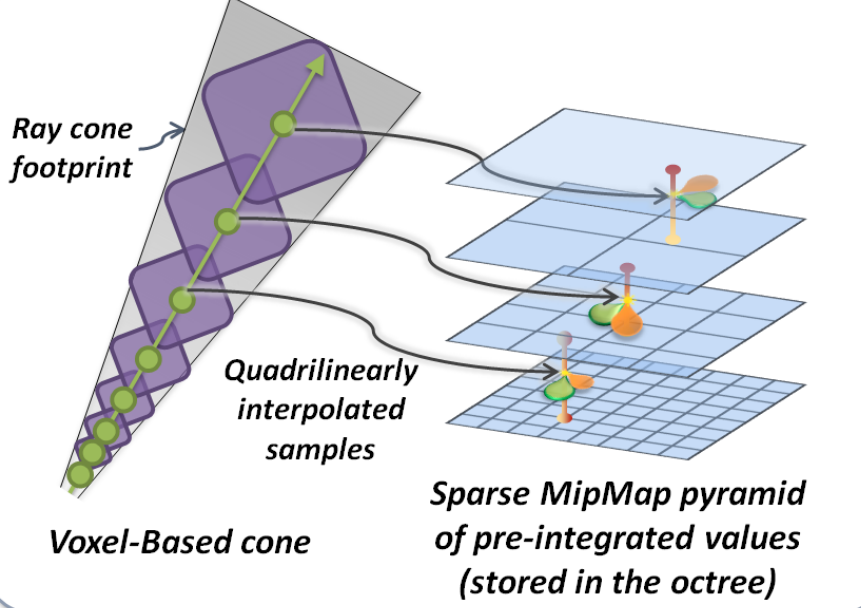
\includegraphics[width=10cm]{voxel-cone-tracing}
	\caption{Voxel Cone Tracing}
\end{figure}

So lassen sich Raytracing-"ahnliche Ergebnisse in Echtzeit erzielen.


\section{Ausblick und Fazit}
Mit heutiger Hardware ist ein Echtzeit-Raytracing einer komplexen Szene und zu einer brauchbaren Bildrate noch nicht m"oglich. Die von mir vorgestellte Methode, bestehend aus Voxelization, der Sparse Voxel Octree-Speicherung und des Voxel Cone Tracing, k"onnen auf heutiger Hardware schon zufriedenstellende Beleuchtungsergebnisse und Bildraten erzielen. 
So kommt dieser Ansatz auch in zuk"unftigen Computerspiel-Engines zum Einsatz. Zum Beispiel nutzt Epic Games diese Methode f"ur die indirekte Beleuchtung und die Ambient Occlusion in der zuk"unftigen Unreal Engine 4. 

Bei der resultierenden Performance kommt es dabei jedoch besonders auf die Gr"o"se des resultierenden Voxelgrids an. Gr"o"sen von $512^3$ und $1024^3$ lassen sich noch bei guter Bildrate erzeugen und beleuchten, bei gr"o"seren Voxelgrids kommt es jedoch, wie beim Raytracing, zu starken Geschwindigkeitseinbu"sen.
 
 
Dieser Ansatz ist jedoch f"ur die n"ahere Zukunft sehr vielversprechend, da auch bei steigenden Aufl"osungen der Szenen noch zufriedenstellende Ergebnisse erzielt werden k"onnen, wohingegen das Raytracing mit der heute zug"anglichen und auch zuk"unftigen Hardware noch einige Jahre brauchen wird, bis es f"ur die Echtzeitdarstellung von 3D-Szenen genutzt werden kann, da hierf"ur eine deutlich schnellere Grafikhardware von N"oten ist.

\end{document}